\subsection{Mixture of Projected Gammas (MPG) Model}
\label{method:mpg}
  In~\ref{method:pmg}, we introduced a projection of two-component mixture of
  gammas (pgm) model.  Here, we go another way, mixing directly on the projected
  gamma distribution at the projection level.  This allows us to establish
  essentially clusters of angular vectors.  Developing the math on this:
\begin{align}
\text{MPG}({\bf \theta}\mid {\bf \lambda}, {\bf \alpha}, {\bf \beta}) &= \sum_{j = 1}^J\lambda_i\text{PG}(\alpha_i,\beta_i) \nonumber \\
&= \int \text{MPG}({\bf \theta}, {\bf \gamma} \mid{\bf \alpha},{\bf \beta})d\gamma \nonumber \\
&= \int \prod_{j = 1}^J\left[\lambda_j\text{PG}({\bf \theta}\mid\alpha_j,\beta_j)\right]^{\gamma_j}\text{d}\gamma \\
&= \int_{\gamma}\int_{r}\lambda_j^{\gamma_j}\prod_{k = 1}^K\text{Ga}(r{\bf y}^{\prime}\mid{\bf \alpha_j},{\bf \beta_j})^{\gamma_j}\lvert\text{Jac}\rvert \text{d}r\text{d}\gamma
\end{align}
letting $\gamma_{ij}$ be an indicator that observation $i$ is in the $j$'th
  mixture component.  From this, we gather the familiar full conditionals.  Let
  $i$ iterate over observations, $j$ iterate over mixture components, and $k$
  iterate over dimensions of the space. Placing a Gamma prior on $\beta$ as
  before, we arrive at a Gamma posterior for $\beta_{jk}$ of the form:
\begin{equation}
  \pi(\beta_{jk}\mid\alpha_{jk}, {\bf r}, {\bf \gamma}) = \text{Ga}\left(\sum_{i = 1}^n \gamma_{ij}\alpha_{jk} + c_0,\sum_{i = 1}^n\gamma_{ij}r_iy_{ik}^{\prime} + d_0\right)
\end{equation}
Integrating $\beta_{jk}$ from $\pi(\alpha_{jk},\beta_{jk}\mid {\bf r}, {\bf \gamma})$,
  we arrive at the full conditional for $\alpha_{jk}$, taking the form:
\begin{equation}
  \pi(\alpha_{jk}\mid\gamma, {\bf r} {\bf \gamma}) \propto \frac{\alpha_{jk}^{a_0 - 1}\prod_{i = 1}^n(r_iy_{ik}^{\prime})^{\gamma_{ij}\alpha_{jk}}}{\Gamma(\alpha_{jk})^{\sum_{i = 1}^n\gamma_{ij}}}\exp\left[-b_0\alpha_{jk}\right]\frac{\Gamma(\alpha_{jk}\sum_i\gamma_{ij} + c_0)}{\left(\sum_ir_iy_{ik}^{\prime} + d_0\right)^{\alpha_{jk}\sum_i\gamma_{ij} + c_0}}
\end{equation}
The radii are generated conditional on the mixture component assignment:
\begin{equation}
\pi(r_i\mid{\bf \gamma}_i, {\bf \alpha}, {\bf \beta}) = \text{Ga}\left(\sum_{j = 1}^J\gamma_{ij}\sum_{k = 1}^K\alpha_{jk}, \sum_{k = 1}^K\left[\sum_{j = 1}^J\gamma_{ij}\beta_{jk}\right]y_{ik}^{\prime}\right)
\end{equation}
Finally, the mixture component indicators ${\bf \gamma}_i$ are generated from
  the Projected Gamma likelihood, rather than introducing the latent $r$'s.
  The full conditional is thus:
\begin{equation}
\pi({\bf \gamma}_i\mid {\bf \lambda},{\bf \alpha},{\bf \beta}) = \text{Multinom}\left(1, \left\lbrace\frac{\lambda_j\text{PG}({\bf y}_i^{\prime}\mid{\bf \alpha}_j,{\bf \beta}_j)}{\sum_{l = 1}^J\lambda_l\text{PG}({\bf y}_i^{\prime}\mid{\bf \alpha}_l,{\bf \beta}_l)}; \hspace{1cm}j = 1,\ldots,J\right\rbrace\right)
\end{equation}
And the full conditional for $\lambda$ is finally:
\begin{equation}
\pi({\bf \lambda}\mid{\bf \gamma}) = \text{Dir}\left(
\left\lbrace \sum_i\gamma_{ij} + a_0; \hspace{1cm}j = 1,\ldots,J\right\rbrace\right)
\end{equation}

The finite mixture of projected gammas model is a rise in complexity versus
  the projected mixture of gammas, and the vanilla projected gamma model.  The
  question is, is that rise justified?  As we can see from \makenote{need to make plot},
  for the most part the MPG model is able to capture the nuance of real data.
  The marginal directional data from the posterior predictive looks very similar
  to that of the empirical.  However, that is true of this dataset.  Is it
  reasonable to stop here?  How do we decide what is an appropriate number of
  mixture components?

Certainly, on an ad-hoc basis one could continue adding mixture components,
  and checking some model selection criterion to find some optimal number of
  components.  Alternatively, using Bayesian non-parametric modelling, we can
  assume a potentially infinite number of components.  We explore that model
  next.

\begin{figure}[h!]
  \label{fig:mpg}
  \centering
  \caption{Posterior Predictive distribution from Mixture of Projected Gammas model with
            15 mixture components, built on declustered IVT data.}
  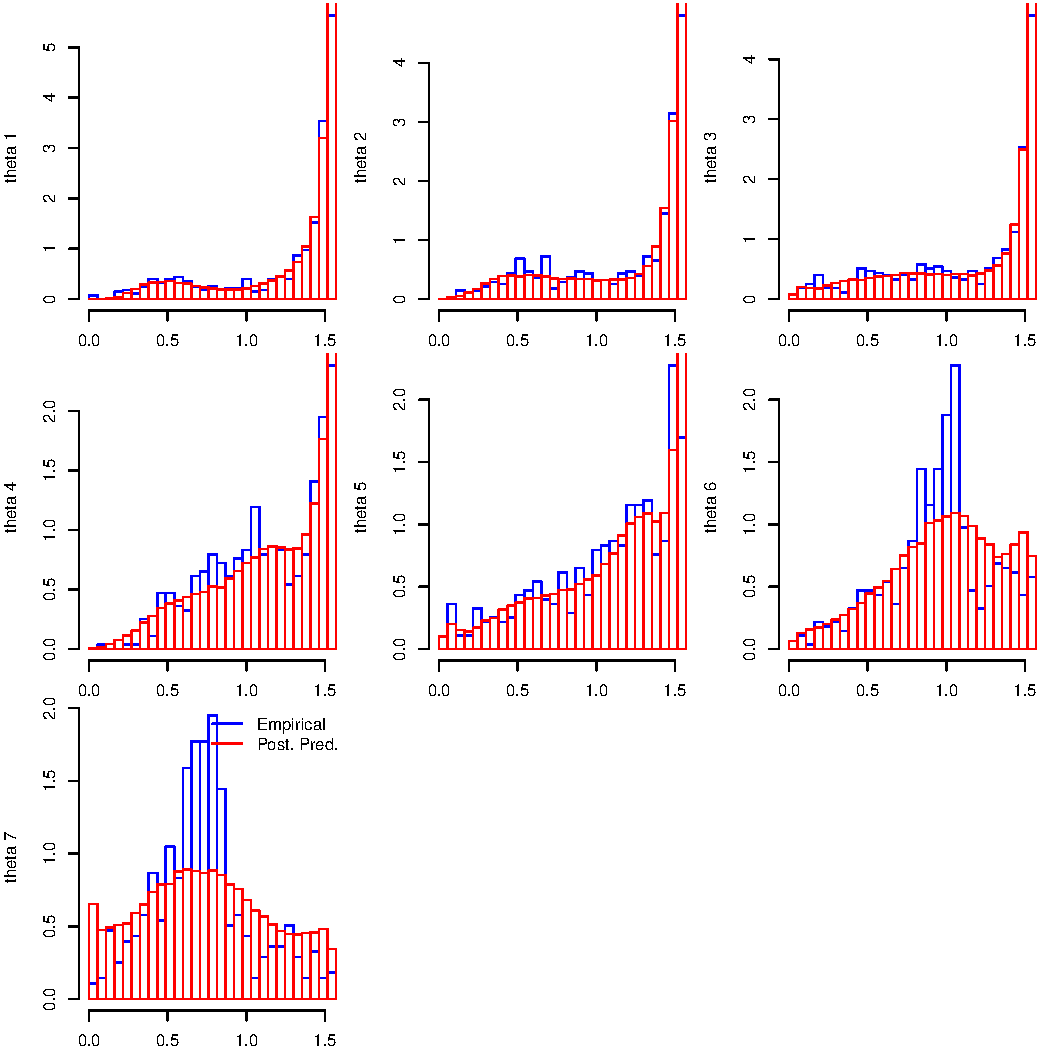
\includegraphics[width=6in]{./images/mpg_15_emp_v_pred_decluster}
\end{figure}

In Figure~\ref{fig:mpg}, we see the posterior predictive distribution generated by the finite
  mixture of projected gammas model.  This model does well in the first $\theta$'s, but we see
  of $\theta_6$ and $\theta_7$, the model has difficulty in fitting the center spikes.  These
  spikes indicate a high degree of extremal dependence between the last 3 columns, so that's
  somewhat a problem.

% EOF
